\documentclass{article}

\usepackage[english]{babel}

% Set page size and margins
\usepackage[a4paper,top=2cm,bottom=2cm,left=3cm,right=3cm,marginparwidth=1.75cm]{geometry}

% Useful packages
\usepackage{amsmath}
\usepackage{enumitem}
\usepackage{graphicx}
\usepackage[colorlinks=true, allcolors=blue]{hyperref}

\title{Multi-Agent Systems Lab - Report 1}
\author{Group 7}

\begin{document}
\maketitle

\section{Question 1}
\begin{enumerate}[label=(\alph*)]
\item 
\begin{figure}[h]
\caption{The Pareto-optimal front}
\centering
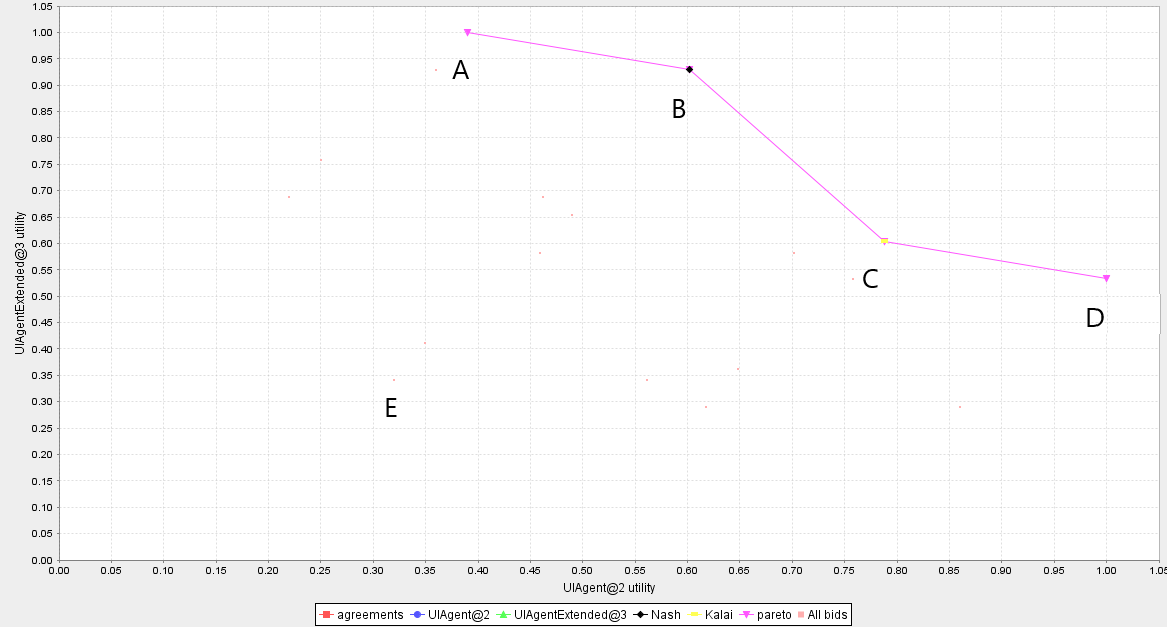
\includegraphics[width=.75\textwidth]{imgs/graph_2}
\end{figure}

When defining the fairest arrangement, there are multiple possibilities. One could argue that the solution that minimizes the difference between the two parties is the fairest. In that case, point E would be the answer. This might be a fair outcome, but it is not a realistic outcome, as it is literally the outcome with the lowest combined utility. Any useful fair outcome therefore should be Pareto-optimal (its front is delimited by the pink line above).

We propose a way to get equal expected utility for both parties, but still get a Pareto-optimal outcome. For this, we need to allow for probability in the outcome of the negotiation. That is, having a certain outcome with 70\% probability and another with 30\% is a valid outcome. Keep in mind that we first throw the weighted coin and then choose an entire outcome, not throw a separate coin for each issue.

Now, the outcome space is no longer a set of points $P$, but the convex hull of $P$. This is because every linear combination of points of $P$ can be achieved by simply having the outcome with the corresponding points and probability.

Note that not all points that were on the Pareto front are still on the Pareto front. In our example, C is no longer on the Pareto front, as taking B with probability 0.4 and D with probability 0.6 will have a higher expected utility for both parties.

Now the Pareto front consists of only outcomes. This is because any linear combination of two previous outcomes is now an outcome as well (and all vertices of $CH(P)$ are in $P$ as well).

Now, we will simply determine a Nash solution for this new problem. This Nash solution is on the Pareto front, so we can simply find the two vertices of the Pareto front that surround the Nash solution, and the fairest solution is a linear combination of those two.

\begin{figure}[ht]
\caption{This theory for our example}
\centering
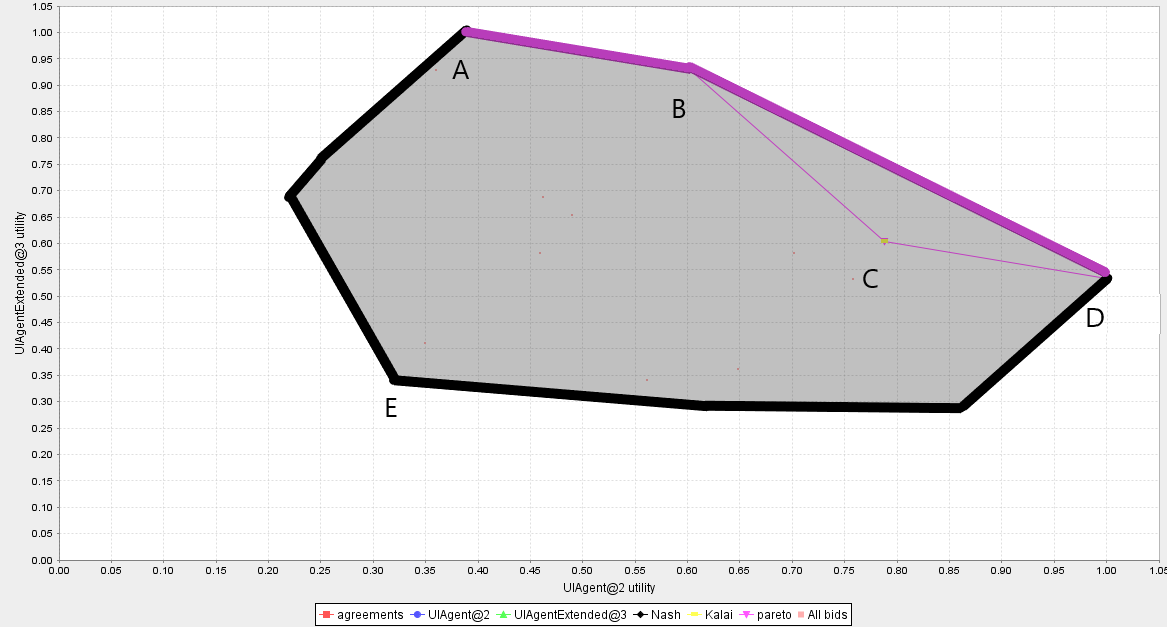
\includegraphics[width=.75\textwidth]{imgs/graph_1} % Lower width means less thick lines!
\end{figure}

In our example, the only vertices of the Pareto front are A, B, and D. A is the outcome where agent B gets everything, D is the outcome where agent A gets everything, and B is the outcome (Milan, 2 weeks, Hostel). This gives the following values for the agents:
\begin{center}
\begin{tabular}{ c c c }
   & Agent A & Agent B \\ 
 A & 3.9 & 10 \\  
 B & 6 & 9.3 \\
 D & 10 & 5.3    
\end{tabular}
\end{center}

Now, it is clear that the Nash solution does not lie on the line segment $AB$, so it lies on the line segment $BD$. Some elementary math tells us that the utility values are $(7.65,7.65)$ and the solution is $0.4125B+0.58875D$, so if we will take $B$ with probability $0.4125$ and $D$ with probability $0.5887$, we get the highest product of expected utilities.

\item We can conclude that the Pareto Optimal Outcome is not (usually) reached, since the bids being made are random. The following figures (3 through 6) graph the Random Bidders negotiations against themselves with varying minimum-targets.

\begin{figure}[ht]
  \minipage{0.50\textwidth}
  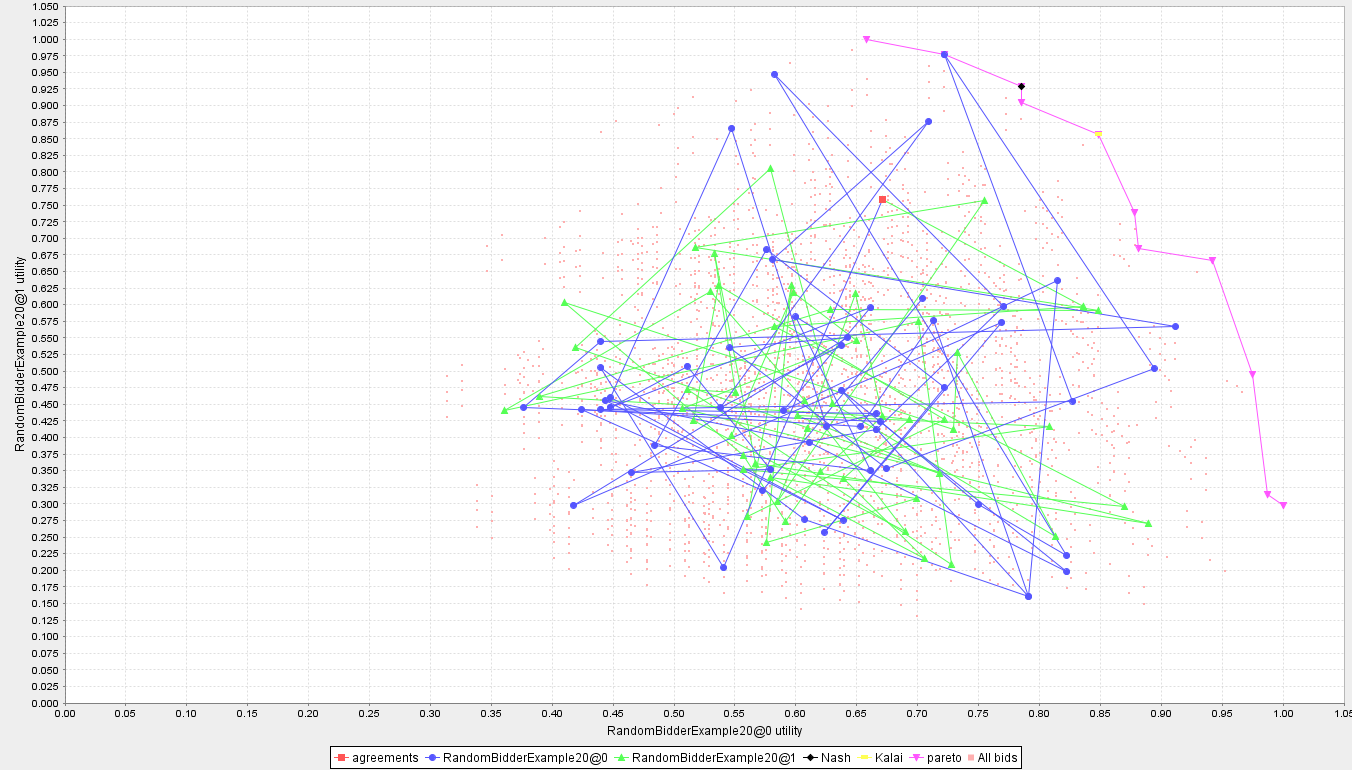
\includegraphics[width=\linewidth]{imgs/rb_20}
  \caption{Minimum Bidding Target = 0.20}
  \endminipage\hfill
  \minipage{0.50\textwidth}
  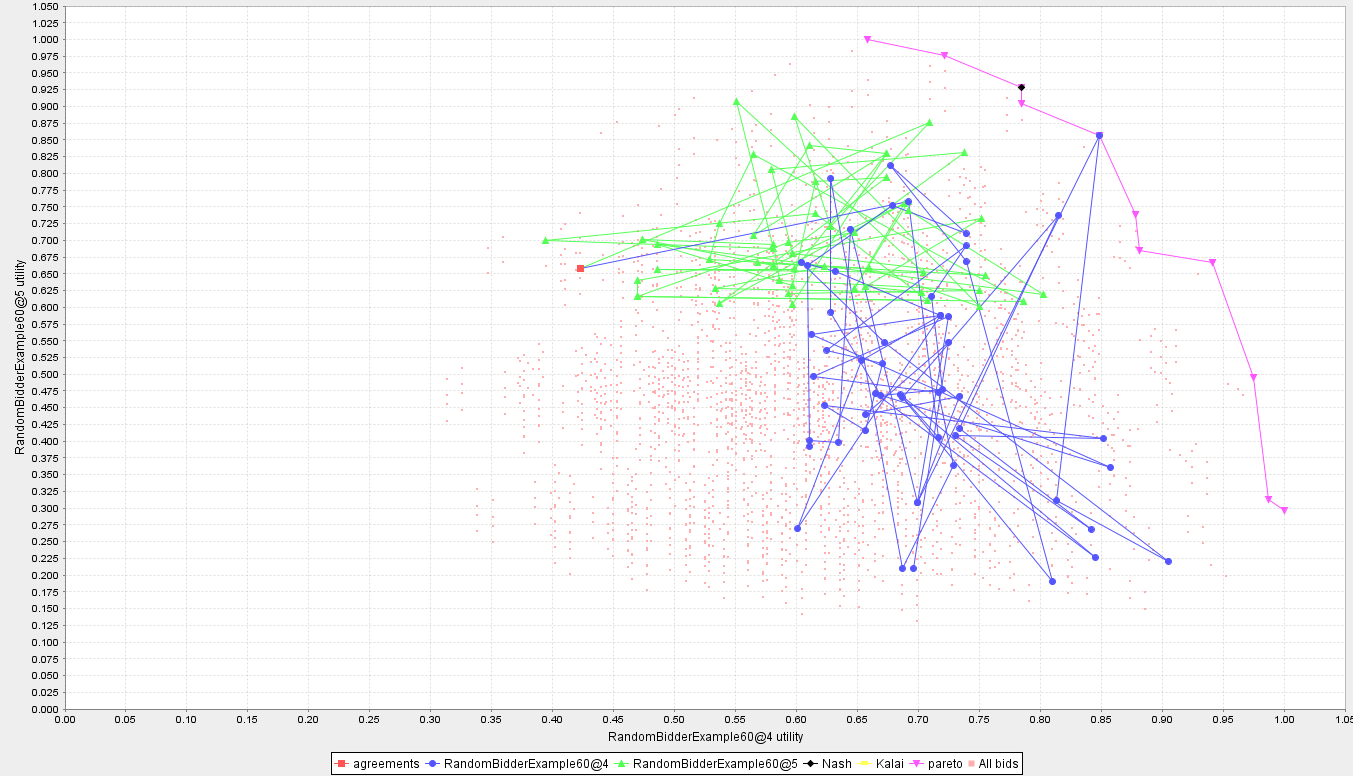
\includegraphics[width=\linewidth]{imgs/rb_60}
  \caption{Minimum Bidding Target = 0.60}
  \endminipage\hfill
\end{figure}

\begin{figure}[ht]
  \minipage{0.50\textwidth}
  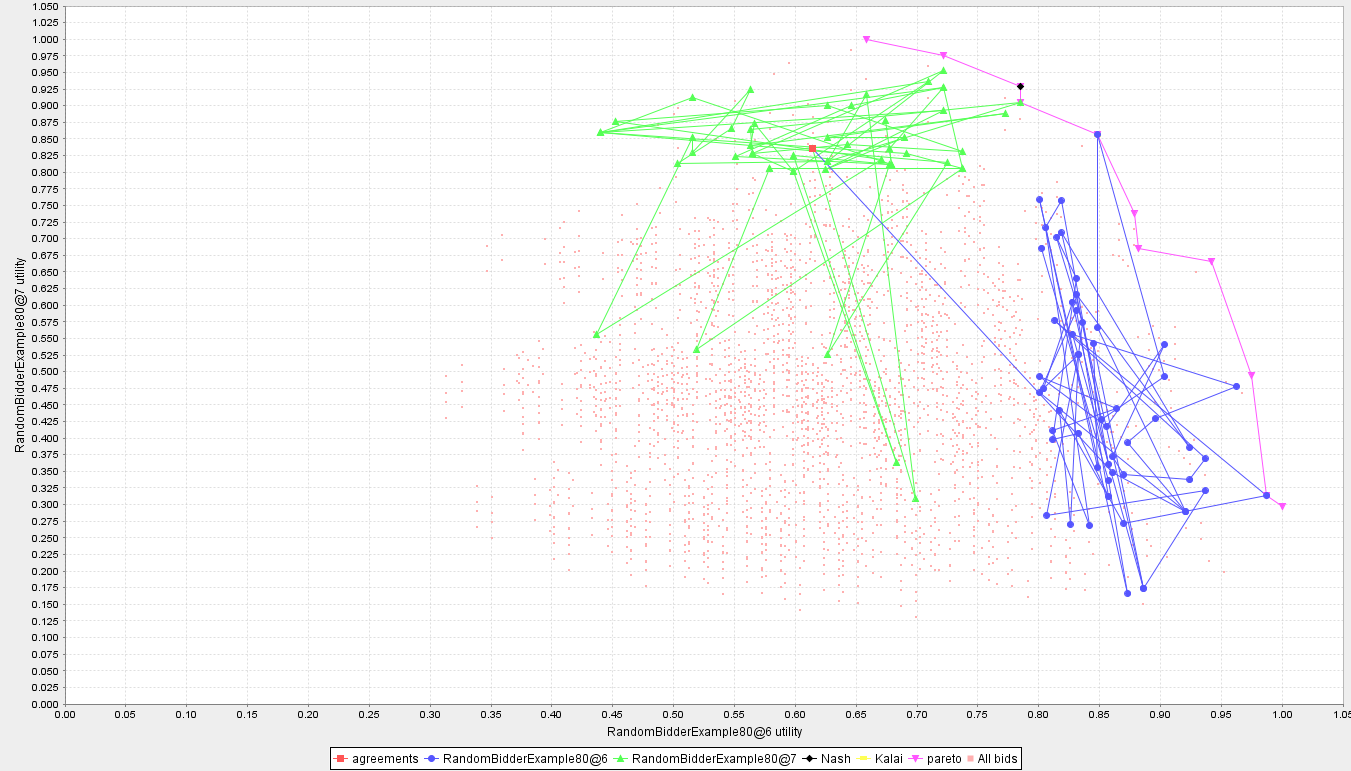
\includegraphics[width=\linewidth]{imgs/rb_80}
  \caption{Minimum Bidding Target = 0.80}
  \endminipage\hfill
  \minipage{0.50\textwidth}
  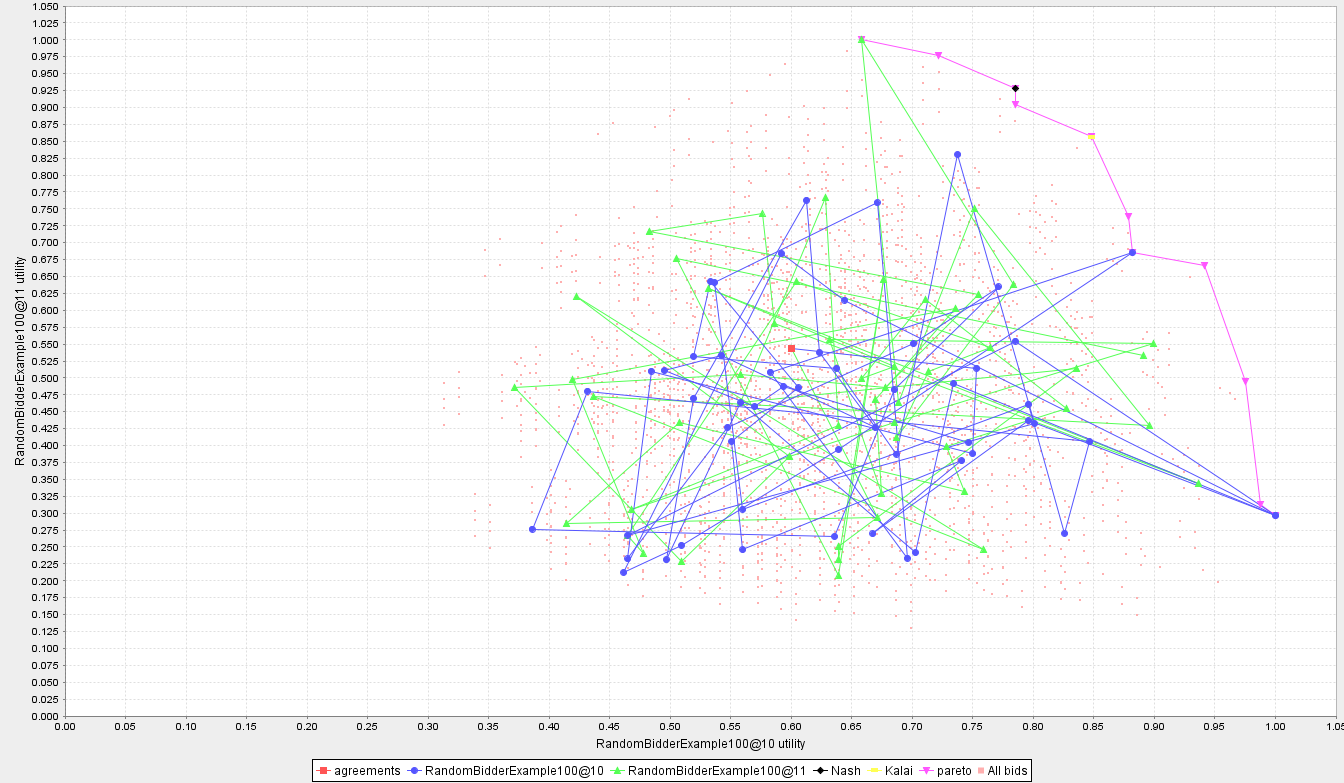
\includegraphics[width=\linewidth]{imgs/rb_100}
  \caption{Minimum Bidding Target = 1.00}
  \endminipage\hfill
\end{figure}

\end{enumerate} % If we need more than two pages we can separate the title page or put figures 1 and 2 in an appendix (in that case make both landscape and very large)
\end{document}